
\documentclass[12pt,a4paper]{article}
\usepackage[utf8]{inputenc}
\usepackage[T1]{fontenc}
\usepackage{mathptmx}
\usepackage[margin=2.54cm]{geometry}
\usepackage{booktabs}
\usepackage{tabularx}
\usepackage{array}
\usepackage{xcolor}
\usepackage{titlesec}
\usepackage{enumitem}
\usepackage{hyperref}
\usepackage{fancyhdr}
\usepackage{setspace}
\usepackage{parskip}
\usepackage{float}
\usepackage{colortbl}
\usepackage{tikz}
\usetikzlibrary{arrows.meta,positioning,shapes.geometric}

\definecolor{navy}{HTML}{1B2A4A}
\definecolor{gold}{HTML}{C49A2A}
\definecolor{dk}{HTML}{2D2D2D}
\definecolor{mg}{HTML}{4A4A4A}
\definecolor{sb}{HTML}{D6E4F0}
\definecolor{sg}{HTML}{DFF0D8}
\definecolor{so}{HTML}{FDEBD0}
\definecolor{sp}{HTML}{E8DAEF}
\definecolor{sr}{HTML}{FADBD8}

\titleformat{\section}{\Large\bfseries\color{navy}}{\thesection}{1em}{}[\vspace{-4pt}{\color{gold}\rule{\textwidth}{1.5pt}}]
\titleformat{\subsection}{\large\bfseries\color{navy}}{\thesubsection}{1em}{}
\titleformat{\subsubsection}{\normalsize\bfseries\color{navy}}{\thesubsubsection}{1em}{}
\setlength{\headheight}{14pt}
\pagestyle{fancy}\fancyhf{}
\fancyhead[L]{\small\color{mg}\textit{Questionnaire Design Framework}}
\fancyhead[R]{\small\color{mg}\textit{AIGGPA, April 2026}}
\fancyfoot[C]{\small\color{mg}\thepage}
\renewcommand{\headrulewidth}{0.4pt}
\hypersetup{colorlinks=true,linkcolor=navy,citecolor=navy,urlcolor=navy}
\setstretch{1.15}
\newcolumntype{L}[1]{>{\raggedright\arraybackslash}p{#1}}
\newcolumntype{C}[1]{>{\centering\arraybackslash}p{#1}}

\begin{document}

% ── TITLE PAGE ──
\begin{titlepage}\centering
\vspace*{2.5cm}
{\color{gold}\rule{0.6\textwidth}{2pt}}\vspace{1cm}

{\Huge\bfseries\color{navy} FRAMEWORK FOR\\[6pt] QUESTIONNAIRE DESIGN}

\vspace{0.5cm}

{\Large\color{dk} A Structured Methodology for Building\\[4pt] Theory-Aligned Research Instruments}

\vspace{1cm}
{\color{gold}\rule{0.6\textwidth}{2pt}}

\vspace{2.5cm}

{\large\color{mg} This document provides a reusable, topic-agnostic framework\\[4pt] for designing survey questionnaires that are rigorously anchored\\[4pt] to theoretical models and produce defensible, analysable data.}

\vspace{2cm}

\begin{tabular}{r l}
\textbf{\color{navy}Prepared By:} & Aryan Kori \\[6pt]
\textbf{\color{navy}Institution:} & AIGGPA, Bhopal \\[6pt]
\textbf{\color{navy}Date:} & April 2026 \\
\end{tabular}

\vfill
{\small\color{mg} Applicable to any mixed-methods or quantitative research design.}
\end{titlepage}

\tableofcontents
\newpage

% ══════════════════════════════════════════
% SECTION 1: THE CORE PRINCIPLE
% ══════════════════════════════════════════
\section{The Core Principle: Every Question Must Be Justified}

The single most important rule of questionnaire design is this: \textbf{if you cannot explain exactly why a question exists in your instrument, it should not be there.}

A poorly designed questionnaire produces data that cannot be analysed, cannot be mapped to a theoretical framework, and cannot defend its findings under academic scrutiny. The framework presented here ensures that every single question in your instrument passes through a rigorous six-layer justification chain --- from the abstract theoretical construct down to the exact phrasing shown to the respondent.

\subsection{The Problem This Framework Solves}

Most student and early-career researchers make one or more of the following mistakes:

\begin{enumerate}[leftmargin=1.5em, itemsep=6pt]
    \item \textbf{``Kitchen Sink'' Syndrome:} Adding questions because they ``seem interesting'' without any theoretical basis. This inflates instrument length, causes respondent fatigue, and produces unusable data.
    \item \textbf{Broken Framework Alignment:} Choosing a theoretical model (e.g., TAM, UTAUT, Maslow) but then writing questions that do not actually measure the constructs defined by that model.
    \item \textbf{Ambiguous Phrasing:} Writing double-barrelled, leading, or vague questions that produce unreliable responses.
    \item \textbf{Scale Mismatch:} Using the wrong data type (e.g., Yes/No when a Likert scale is needed for regression analysis), making the data incompatible with the planned statistical tests.
    \item \textbf{No Audit Trail:} Being unable to defend, in a viva or review, \textit{why} a specific question is in the instrument and what it contributes to the analysis.
\end{enumerate}

This framework eliminates all five problems by forcing every question through a structured design pipeline.

\newpage

% ══════════════════════════════════════════
% SECTION 2: THE SIX-PARAMETER MODEL
% ══════════════════════════════════════════
\section{The Six-Parameter Question Design Model}

Every question in your instrument must be defined by exactly six parameters. Think of these as layers in a funnel --- each layer narrows the focus from abstract theory to concrete measurement.

\vspace{12pt}

\begin{center}
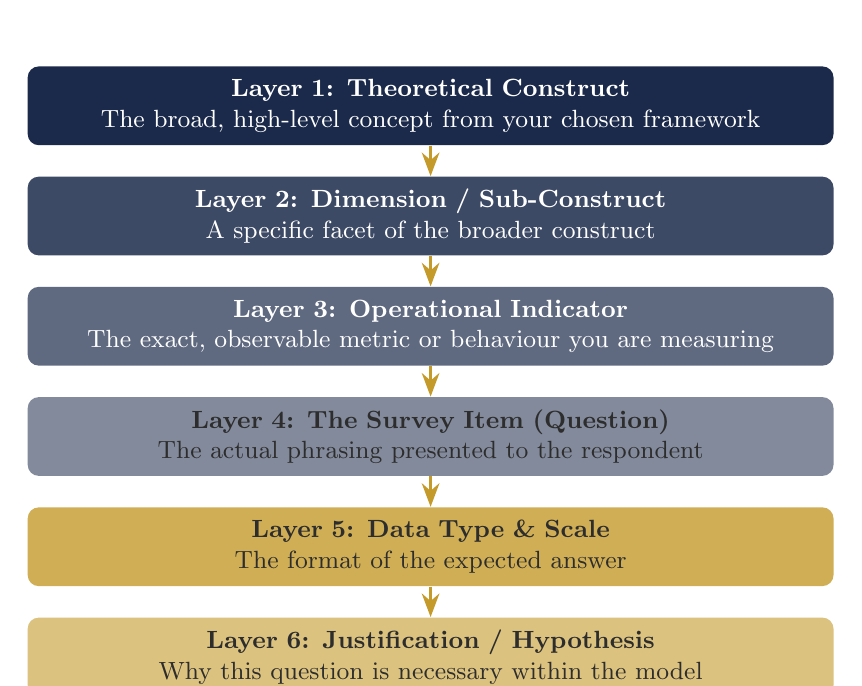
\begin{tikzpicture}[
    every node/.style={font=\small, text=white, minimum height=1cm, text width=10cm, align=center},
    arrow/.style={-{Stealth[length=3mm]}, thick, color=gold}
]
\node[fill=navy, rounded corners=4pt] (L1) at (0, 0) {\textbf{Layer 1: Theoretical Construct}\\The broad, high-level concept from your chosen framework};
\node[fill=navy!85, rounded corners=4pt] (L2) at (0, -1.4) {\textbf{Layer 2: Dimension / Sub-Construct}\\A specific facet of the broader construct};
\node[fill=navy!70, rounded corners=4pt] (L3) at (0, -2.8) {\textbf{Layer 3: Operational Indicator}\\The exact, observable metric or behaviour you are measuring};
\node[fill=navy!55, rounded corners=4pt, text=dk] (L4) at (0, -4.2) {\textbf{Layer 4: The Survey Item (Question)}\\The actual phrasing presented to the respondent};
\node[fill=gold!80, rounded corners=4pt, text=dk] (L5) at (0, -5.6) {\textbf{Layer 5: Data Type \& Scale}\\The format of the expected answer};
\node[fill=gold!60, rounded corners=4pt, text=dk] (L6) at (0, -7.0) {\textbf{Layer 6: Justification / Hypothesis}\\Why this question is necessary within the model};
\draw[arrow] (L1.south) -- (L2.north);
\draw[arrow] (L2.south) -- (L3.north);
\draw[arrow] (L3.south) -- (L4.north);
\draw[arrow] (L4.south) -- (L5.north);
\draw[arrow] (L5.south) -- (L6.north);
\end{tikzpicture}
\end{center}

\vspace{8pt}

The following subsections explain each layer in detail.

\newpage

\subsection{Layer 1: Theoretical Construct}

\begin{table}[H]\centering\small
\begin{tabularx}{\textwidth}{L{3cm} X}
\toprule
\textbf{Definition} & The broad, high-level concept from your chosen theoretical framework. \\
\midrule
\textbf{Framework Role} & Anchors a section of the questionnaire to a specific pillar of the framework. \\
\midrule
\textbf{Why It Matters} & Ensures that all major theoretical pillars are covered and prevents scope creep. If a question does not map to any construct in your framework, it does not belong in the instrument. \\
\midrule
\textbf{Example} & In UTAUT: ``Facilitating Conditions'' (FC). In Maslow's Hierarchy: ``Safety Needs''. In Herzberg's Two-Factor: ``Hygiene Factors''. \\
\midrule
\textbf{Common Mistake} & Writing questions that ``feel relevant'' but do not map to any construct. These produce orphan data that cannot be analysed within the framework. \\
\bottomrule
\end{tabularx}
\end{table}

\subsection{Layer 2: Dimension / Sub-Construct}

\begin{table}[H]\centering\small
\begin{tabularx}{\textwidth}{L{3cm} X}
\toprule
\textbf{Definition} & A specific facet of the broader construct. Most frameworks break main ideas into smaller categories. \\
\midrule
\textbf{Framework Role} & Maps directly to the sub-categories or variables defined in the literature. \\
\midrule
\textbf{Why It Matters} & Abstract constructs are too vague to measure directly. Breaking them into dimensions isolates specific mechanisms and enables finer diagnostic analysis. \\
\midrule
\textbf{Example} & Construct: ``Facilitating Conditions'' $\rightarrow$ Dimension: ``Hardware Infrastructure'' or ``Technical Support Availability''. \\
\midrule
\textbf{Common Mistake} & Treating the entire construct as one monolithic block and writing only one generic question for it, losing all diagnostic power. \\
\bottomrule
\end{tabularx}
\end{table}

\subsection{Layer 3: Operational Indicator}

\begin{table}[H]\centering\small
\begin{tabularx}{\textwidth}{L{3cm} X}
\toprule
\textbf{Definition} & The exact, observable metric or behaviour you are trying to capture. \\
\midrule
\textbf{Framework Role} & Acts as the bridge between the framework's theory and the practical data model. \\
\midrule
\textbf{Why It Matters} & You need a defined, measurable target to structure the question around so the resulting data is statistically useful and operationally meaningful. \\
\midrule
\textbf{Example} & Dimension: ``Hardware Infrastructure'' $\rightarrow$ Indicator: ``Number of dedicated digital devices available per employee at their workstation''. \\
\midrule
\textbf{Common Mistake} & Jumping from a dimension directly to a question without defining what, exactly, you are measuring. This leads to vague, double-barrelled questions. \\
\bottomrule
\end{tabularx}
\end{table}

\subsection{Layer 4: The Survey Item (Question)}

\begin{table}[H]\centering\small
\begin{tabularx}{\textwidth}{L{3cm} X}
\toprule
\textbf{Definition} & The actual phrasing presented to the respondent. Must be unambiguous, single-barrelled, and neutral. \\
\midrule
\textbf{Framework Role} & Translates the operational indicator into human-readable language that a non-expert respondent can answer accurately. \\
\midrule
\textbf{Why It Matters} & Phrasing determines data quality. If the question does not accurately reflect the indicator, the entire framework alignment breaks. \\
\midrule
\textbf{Example} & Indicator: ``Number of dedicated digital devices'' $\rightarrow$ Item: ``What digital devices are available at your personal workstation? (Select all that apply: Desktop / Laptop / Tablet / Smartphone / None)'' \\
\midrule
\textbf{Rules} & (1)~Single-barrelled: ask only one thing. (2)~Avoid leading language. (3)~Avoid jargon the respondent may not understand. (4)~Specify the time frame if applicable. (5)~Provide exhaustive, mutually exclusive response options. \\
\bottomrule
\end{tabularx}
\end{table}

\subsection{Layer 5: Data Type \& Scale}

\begin{table}[H]\centering\small
\begin{tabularx}{\textwidth}{L{3cm} X}
\toprule
\textbf{Definition} & The format of the expected answer --- Likert scale, categorical, numeric/ratio, multi-select, or open-ended. \\
\midrule
\textbf{Framework Role} & Dictates how the data will be coded and analysed against the framework's hypotheses. \\
\midrule
\textbf{Why It Matters} & Different analytical methods require specific data types. You need continuous/ordinal data for regression and correlation; categorical data for chi-square; ratio data for means and t-tests. Choosing the wrong scale makes your planned analysis impossible. \\
\midrule
\textbf{Scale Types} & \textbf{Likert (Ordinal):} 5-point or 7-point agreement/frequency scales. \newline \textbf{Categorical (Nominal):} Mutually exclusive groups (Yes/No, department names). \newline \textbf{Numeric (Ratio):} Exact counts (years, hours, number of sessions). \newline \textbf{Multi-Select:} Checklists where multiple options can be selected. \newline \textbf{Open-Ended:} Free-text for qualitative thematic analysis. \\
\midrule
\textbf{Common Mistake} & Using Yes/No when a Likert scale is needed, or using open-ended when a structured scale would provide more analysable data. \\
\bottomrule
\end{tabularx}
\end{table}

\subsection{Layer 6: Justification / Hypothesis}

\begin{table}[H]\centering\small
\begin{tabularx}{\textwidth}{L{3cm} X}
\toprule
\textbf{Definition} & A brief note explaining exactly what this question proves or disproves within the context of the model. \\
\midrule
\textbf{Framework Role} & Explicitly states the expected relationship between this item and the framework's outcome variable or hypothesis. \\
\midrule
\textbf{Why It Matters} & Provides a defence for why the question is necessary. If you cannot justify a question's specific purpose within the model, it should be removed. This is the ultimate ``so what?'' test. \\
\midrule
\textbf{Example} & ``Device availability is a direct measure of Facilitating Conditions; low FC scores are hypothesised to reduce technology adoption regardless of user attitudes (Venkatesh et al., 2003).'' \\
\midrule
\textbf{Common Mistake} & Including questions with no clear analytical purpose. If a question's data will never appear in any table, chart, or finding in your report, it is wasting the respondent's time. \\
\bottomrule
\end{tabularx}
\end{table}

\newpage

% ══════════════════════════════════════════
% SECTION 3: THE DESIGN WORKFLOW
% ══════════════════════════════════════════
\section{The Design Workflow: Step-by-Step Process}

Follow these steps in order when building your questionnaire from scratch.

\subsection{Step 1: Identify Your Theoretical Framework}

Before writing a single question, decide on the framework your study is built on. Common frameworks include:

\begin{table}[H]\centering\small
\begin{tabularx}{\textwidth}{L{4cm} L{3cm} X}
\toprule
\textbf{Framework} & \textbf{Domain} & \textbf{Core Constructs} \\
\midrule
TAM (Davis, 1989) & Technology Adoption & Perceived Usefulness, Perceived Ease of Use \\[4pt]
UTAUT (Venkatesh et al., 2003) & Technology Adoption & Performance Expectancy, Effort Expectancy, Social Influence, Facilitating Conditions \\[4pt]
Maslow's Hierarchy & Motivation / Needs & Physiological, Safety, Belonging, Esteem, Self-Actualisation \\[4pt]
Herzberg Two-Factor & Job Satisfaction & Hygiene Factors, Motivators \\[4pt]
SERVQUAL & Service Quality & Tangibles, Reliability, Responsiveness, Assurance, Empathy \\
\bottomrule
\end{tabularx}
\end{table}

Your framework determines which constructs exist. Every question must trace back to one of these constructs.

\subsection{Step 2: Decompose Constructs into Dimensions}

For each construct, identify 2--4 dimensions based on the literature. This is where you do your literature review work.

\textbf{Template:}
\begin{quote}
Construct: [Name] $\rightarrow$ Dimension 1: [Specific facet] $\rightarrow$ Dimension 2: [Another facet] $\rightarrow$ ...
\end{quote}

\subsection{Step 3: Define Operational Indicators for Each Dimension}

For each dimension, ask: ``What specific, observable thing would I need to measure to assess this dimension?'' Write 1--3 indicators per dimension.

\subsection{Step 4: Write the Survey Items}

For each indicator, write one question following these rules:
\begin{itemize}[leftmargin=1.5em, itemsep=3pt]
    \item \textbf{Single-barrelled:} One concept per question. Never ``Do you find the tool useful \textit{and} easy to use?''
    \item \textbf{Neutral phrasing:} Avoid leading the respondent toward a particular answer.
    \item \textbf{Plain language:} Write for your actual respondent, not for an academic audience.
    \item \textbf{Specific time frame:} ``In the last 12 months'' is better than ``generally''.
    \item \textbf{Exhaustive options:} All possible answers must be covered, including ``Other'' and ``Not applicable''.
\end{itemize}

\subsection{Step 5: Assign Data Types \& Scales}

Match each question to the appropriate scale based on your planned analysis:

\begin{table}[H]\centering\small
\begin{tabularx}{\textwidth}{L{3.5cm} L{4cm} X}
\toprule
\textbf{If You Need To\ldots} & \textbf{Use This Scale} & \textbf{Compatible Analysis} \\
\midrule
Measure attitudes or perceptions & 5-point Likert (Ordinal) & Median, mode, Mann-Whitney U, Kruskal-Wallis, Cronbach's $\alpha$ \\[4pt]
Classify respondents into groups & Categorical (Nominal) & Frequency, cross-tabulation, chi-square \\[4pt]
Count exact quantities & Numeric (Ratio) & Mean, SD, t-test, ANOVA, regression \\[4pt]
Allow multiple selections & Multi-select checklist & Frequency per option, percentage analysis \\[4pt]
Capture rich qualitative data & Open-ended text & Thematic analysis (Braun \& Clarke, 2006) \\
\bottomrule
\end{tabularx}
\end{table}

\subsection{Step 6: Write the Justification}

For every question, complete this sentence:

\begin{quote}
\textit{``This question measures [indicator] within the [dimension] facet of [construct]. The data produced will be used to [specific analytical purpose]. Without this question, the study would be unable to [specific gap].''}
\end{quote}

If you cannot complete this sentence convincingly, the question should be removed.

\newpage

% ══════════════════════════════════════════
% SECTION 4: THE QUESTION CARD TEMPLATE
% ══════════════════════════════════════════
\section{The Question Card Template}

Use this template for every question in your instrument. It serves as both a design tool and a documentation record.

\vspace{8pt}

\noindent\begin{tabularx}{\textwidth}{@{}>{\columncolor{sb}\bfseries\small}L{3.2cm}|X@{}}
\arrayrulecolor{navy}\hline
Theoretical Construct & [Name of the construct from your framework] \\
Dimension & [Specific facet/sub-construct] \\
Operational Indicator & [The exact observable metric or behaviour] \\
\arrayrulecolor{gold}\hline
\rowcolor{white}\textbf{\color{navy}Survey Item} & \textbf{\color{navy}[The actual question, written in plain language]} \\
\arrayrulecolor{gold}\hline
Data Type \& Scale & [Likert / Categorical / Numeric / Multi-select / Open-ended --- with specific options] \\
Justification & \textit{[Why this question exists, what it measures, what analysis it feeds, and what academic source supports it]} \\
\arrayrulecolor{navy}\hline
\end{tabularx}

\vspace{12pt}

\noindent\textbf{Worked Example (using UTAUT):}

\vspace{8pt}

\noindent\begin{tabularx}{\textwidth}{@{}>{\columncolor{sg}\bfseries\small}L{3.2cm}|X@{}}
\arrayrulecolor{navy}\hline
Theoretical Construct & Facilitating Conditions (FC) \\
Dimension & Hardware Infrastructure \\
Operational Indicator & Availability of dedicated digital devices at employee workstation \\
\arrayrulecolor{gold}\hline
\rowcolor{white}\textbf{\color{navy}Survey Item} & \textbf{\color{navy}What digital devices are available at your personal workstation? (Select all: Desktop / Laptop / Tablet / Smartphone / None)} \\
\arrayrulecolor{gold}\hline
Data Type \& Scale & Multi-select Checklist (Nominal) \\
Justification & \textit{FC requires that organisational infrastructure exists to support system use; device availability is the most direct measure of hardware FC (Venkatesh et al., 2003). Low device counts indicate insufficient FC, hypothesised to reduce adoption regardless of individual attitudes.} \\
\arrayrulecolor{navy}\hline
\end{tabularx}

\newpage

% ══════════════════════════════════════════
% SECTION 5: QUALITY CHECKLIST
% ══════════════════════════════════════════
\section{Quality Checklist Before Finalising}

Run every question through this checklist before including it in your final instrument.

\begin{table}[H]\centering\small
\begin{tabularx}{\textwidth}{C{0.8cm} L{4.5cm} X}
\toprule
\textbf{\#} & \textbf{Check} & \textbf{What to Look For} \\
\midrule
1 & Construct Mapping & Does this question map to a specific construct in your framework? \\[4pt]
2 & Dimension Specificity & Is the dimension narrow enough to isolate a specific mechanism? \\[4pt]
3 & Indicator Clarity & Is the indicator observable and measurable, not abstract? \\[4pt]
4 & Single-Barrelled & Does the question ask only one thing? \\[4pt]
5 & Neutral Phrasing & Is the question free from leading or loaded language? \\[4pt]
6 & Respondent Appropriate & Can your actual respondent (not a fellow researcher) understand it? \\[4pt]
7 & Scale--Analysis Match & Does the chosen scale produce data compatible with your planned statistical tests? \\[4pt]
8 & Justification Test & Can you explain in one sentence why this question must be in the instrument? \\[4pt]
9 & Redundancy Check & Is this question already covered by another item? If so, merge or remove. \\[4pt]
10 & Construct Coverage & Have all constructs in your framework been addressed by at least 2--3 questions? \\
\bottomrule
\end{tabularx}
\end{table}

\section{Reliability \& Validity Considerations}

Once your instrument is designed, you must test it before deployment:

\begin{enumerate}[leftmargin=1.5em, itemsep=6pt]
    \item \textbf{Content Validity:} Have 2--3 subject-matter experts review whether your questions adequately cover all constructs and dimensions.
    \item \textbf{Face Validity:} Pilot-test with 5--10 respondents similar to your sample. Ask them if questions are clear and unambiguous.
    \item \textbf{Internal Consistency (Cronbach's $\alpha$):} After pilot data collection, run Cronbach's Alpha on each construct sub-scale. Threshold: $\alpha \geq 0.70$ (Cronbach, 1951; Tavakol \& Dennick, 2011).
    \item \textbf{Construct Validity:} Ensure items measuring the same construct correlate with each other (convergent validity) and do not correlate with items from different constructs (discriminant validity).
\end{enumerate}

\newpage

% ══════════════════════════════════════════
% REFERENCES
% ══════════════════════════════════════════
\section*{References}
\addcontentsline{toc}{section}{References}

\begin{enumerate}[leftmargin=1.5em,itemsep=3pt,label={[\arabic*]}]
    \item Braun, V., \& Clarke, V. (2006). Using thematic analysis in psychology. \textit{Qualitative Research in Psychology}, 3(2), 77--101.
    \item Cronbach, L. J. (1951). Coefficient alpha and the internal structure of tests. \textit{Psychometrika}, 16(3), 297--334.
    \item Davis, F. D. (1989). Perceived usefulness, perceived ease of use, and user acceptance of information technology. \textit{MIS Quarterly}, 13(3), 319--340.
    \item Field, A. (2018). \textit{Discovering Statistics Using IBM SPSS Statistics} (5th ed.). SAGE Publications.
    \item Parasuraman, A., Zeithaml, V. A., \& Berry, L. L. (1988). SERVQUAL: A multiple-item scale for measuring consumer perceptions of service quality. \textit{Journal of Retailing}, 64(1), 12--40.
    \item Tavakol, M., \& Dennick, R. (2011). Making sense of Cronbach's alpha. \textit{International Journal of Medical Education}, 2, 53--55.
    \item Venkatesh, V., Morris, M. G., Davis, G. B., \& Davis, F. D. (2003). User acceptance of information technology: Toward a unified view. \textit{MIS Quarterly}, 27(3), 425--478.
\end{enumerate}

\end{document}
